% Options for packages loaded elsewhere
\PassOptionsToPackage{unicode}{hyperref}
\PassOptionsToPackage{hyphens}{url}
%
\documentclass[
]{article}
\title{Vaccination Rate Mini-Project: class17}
\author{Chloe J. Welch}
\date{11/26/2021}

\usepackage{amsmath,amssymb}
\usepackage{lmodern}
\usepackage{iftex}
\ifPDFTeX
  \usepackage[T1]{fontenc}
  \usepackage[utf8]{inputenc}
  \usepackage{textcomp} % provide euro and other symbols
\else % if luatex or xetex
  \usepackage{unicode-math}
  \defaultfontfeatures{Scale=MatchLowercase}
  \defaultfontfeatures[\rmfamily]{Ligatures=TeX,Scale=1}
\fi
% Use upquote if available, for straight quotes in verbatim environments
\IfFileExists{upquote.sty}{\usepackage{upquote}}{}
\IfFileExists{microtype.sty}{% use microtype if available
  \usepackage[]{microtype}
  \UseMicrotypeSet[protrusion]{basicmath} % disable protrusion for tt fonts
}{}
\makeatletter
\@ifundefined{KOMAClassName}{% if non-KOMA class
  \IfFileExists{parskip.sty}{%
    \usepackage{parskip}
  }{% else
    \setlength{\parindent}{0pt}
    \setlength{\parskip}{6pt plus 2pt minus 1pt}}
}{% if KOMA class
  \KOMAoptions{parskip=half}}
\makeatother
\usepackage{xcolor}
\IfFileExists{xurl.sty}{\usepackage{xurl}}{} % add URL line breaks if available
\IfFileExists{bookmark.sty}{\usepackage{bookmark}}{\usepackage{hyperref}}
\hypersetup{
  pdftitle={Vaccination Rate Mini-Project: class17},
  pdfauthor={Chloe J. Welch},
  hidelinks,
  pdfcreator={LaTeX via pandoc}}
\urlstyle{same} % disable monospaced font for URLs
\usepackage[margin=1in]{geometry}
\usepackage{color}
\usepackage{fancyvrb}
\newcommand{\VerbBar}{|}
\newcommand{\VERB}{\Verb[commandchars=\\\{\}]}
\DefineVerbatimEnvironment{Highlighting}{Verbatim}{commandchars=\\\{\}}
% Add ',fontsize=\small' for more characters per line
\usepackage{framed}
\definecolor{shadecolor}{RGB}{248,248,248}
\newenvironment{Shaded}{\begin{snugshade}}{\end{snugshade}}
\newcommand{\AlertTok}[1]{\textcolor[rgb]{0.94,0.16,0.16}{#1}}
\newcommand{\AnnotationTok}[1]{\textcolor[rgb]{0.56,0.35,0.01}{\textbf{\textit{#1}}}}
\newcommand{\AttributeTok}[1]{\textcolor[rgb]{0.77,0.63,0.00}{#1}}
\newcommand{\BaseNTok}[1]{\textcolor[rgb]{0.00,0.00,0.81}{#1}}
\newcommand{\BuiltInTok}[1]{#1}
\newcommand{\CharTok}[1]{\textcolor[rgb]{0.31,0.60,0.02}{#1}}
\newcommand{\CommentTok}[1]{\textcolor[rgb]{0.56,0.35,0.01}{\textit{#1}}}
\newcommand{\CommentVarTok}[1]{\textcolor[rgb]{0.56,0.35,0.01}{\textbf{\textit{#1}}}}
\newcommand{\ConstantTok}[1]{\textcolor[rgb]{0.00,0.00,0.00}{#1}}
\newcommand{\ControlFlowTok}[1]{\textcolor[rgb]{0.13,0.29,0.53}{\textbf{#1}}}
\newcommand{\DataTypeTok}[1]{\textcolor[rgb]{0.13,0.29,0.53}{#1}}
\newcommand{\DecValTok}[1]{\textcolor[rgb]{0.00,0.00,0.81}{#1}}
\newcommand{\DocumentationTok}[1]{\textcolor[rgb]{0.56,0.35,0.01}{\textbf{\textit{#1}}}}
\newcommand{\ErrorTok}[1]{\textcolor[rgb]{0.64,0.00,0.00}{\textbf{#1}}}
\newcommand{\ExtensionTok}[1]{#1}
\newcommand{\FloatTok}[1]{\textcolor[rgb]{0.00,0.00,0.81}{#1}}
\newcommand{\FunctionTok}[1]{\textcolor[rgb]{0.00,0.00,0.00}{#1}}
\newcommand{\ImportTok}[1]{#1}
\newcommand{\InformationTok}[1]{\textcolor[rgb]{0.56,0.35,0.01}{\textbf{\textit{#1}}}}
\newcommand{\KeywordTok}[1]{\textcolor[rgb]{0.13,0.29,0.53}{\textbf{#1}}}
\newcommand{\NormalTok}[1]{#1}
\newcommand{\OperatorTok}[1]{\textcolor[rgb]{0.81,0.36,0.00}{\textbf{#1}}}
\newcommand{\OtherTok}[1]{\textcolor[rgb]{0.56,0.35,0.01}{#1}}
\newcommand{\PreprocessorTok}[1]{\textcolor[rgb]{0.56,0.35,0.01}{\textit{#1}}}
\newcommand{\RegionMarkerTok}[1]{#1}
\newcommand{\SpecialCharTok}[1]{\textcolor[rgb]{0.00,0.00,0.00}{#1}}
\newcommand{\SpecialStringTok}[1]{\textcolor[rgb]{0.31,0.60,0.02}{#1}}
\newcommand{\StringTok}[1]{\textcolor[rgb]{0.31,0.60,0.02}{#1}}
\newcommand{\VariableTok}[1]{\textcolor[rgb]{0.00,0.00,0.00}{#1}}
\newcommand{\VerbatimStringTok}[1]{\textcolor[rgb]{0.31,0.60,0.02}{#1}}
\newcommand{\WarningTok}[1]{\textcolor[rgb]{0.56,0.35,0.01}{\textbf{\textit{#1}}}}
\usepackage{longtable,booktabs,array}
\usepackage{calc} % for calculating minipage widths
% Correct order of tables after \paragraph or \subparagraph
\usepackage{etoolbox}
\makeatletter
\patchcmd\longtable{\par}{\if@noskipsec\mbox{}\fi\par}{}{}
\makeatother
% Allow footnotes in longtable head/foot
\IfFileExists{footnotehyper.sty}{\usepackage{footnotehyper}}{\usepackage{footnote}}
\makesavenoteenv{longtable}
\usepackage{graphicx}
\makeatletter
\def\maxwidth{\ifdim\Gin@nat@width>\linewidth\linewidth\else\Gin@nat@width\fi}
\def\maxheight{\ifdim\Gin@nat@height>\textheight\textheight\else\Gin@nat@height\fi}
\makeatother
% Scale images if necessary, so that they will not overflow the page
% margins by default, and it is still possible to overwrite the defaults
% using explicit options in \includegraphics[width, height, ...]{}
\setkeys{Gin}{width=\maxwidth,height=\maxheight,keepaspectratio}
% Set default figure placement to htbp
\makeatletter
\def\fps@figure{htbp}
\makeatother
\setlength{\emergencystretch}{3em} % prevent overfull lines
\providecommand{\tightlist}{%
  \setlength{\itemsep}{0pt}\setlength{\parskip}{0pt}}
\setcounter{secnumdepth}{-\maxdimen} % remove section numbering
\ifLuaTeX
  \usepackage{selnolig}  % disable illegal ligatures
\fi

\begin{document}
\maketitle

\hypertarget{getting-started}{%
\section{Getting started}\label{getting-started}}

We will start by downloading the most recently dated ``Statewide
COVID-19 Vaccines Administered by ZIP Code'' CSV file from:
\url{https://data.ca.gov/dataset/covid-19-vaccine-progress-dashboard-data-by-zip-code}

Be sure to move your downloaded CSV file to your project directory and
then read/import into an R object called vax. We will use this data to
answer all the questions below.

\begin{Shaded}
\begin{Highlighting}[]
\CommentTok{\# Import vaccination data}
\NormalTok{vax }\OtherTok{\textless{}{-}} \FunctionTok{read.csv}\NormalTok{(}\StringTok{"vaxdata.csv"}\NormalTok{)}
\FunctionTok{head}\NormalTok{(vax)}
\end{Highlighting}
\end{Shaded}

\begin{verbatim}
##   as_of_date zip_code_tabulation_area local_health_jurisdiction         county
## 1 2021-01-05                    92395            San Bernardino San Bernardino
## 2 2021-01-05                    93206                      Kern           Kern
## 3 2021-01-05                    91006               Los Angeles    Los Angeles
## 4 2021-01-05                    91901                 San Diego      San Diego
## 5 2021-01-05                    92230                 Riverside      Riverside
## 6 2021-01-05                    92662                    Orange         Orange
##   vaccine_equity_metric_quartile                 vem_source
## 1                              1 Healthy Places Index Score
## 2                              1 Healthy Places Index Score
## 3                              3 Healthy Places Index Score
## 4                              3 Healthy Places Index Score
## 5                              1 Healthy Places Index Score
## 6                              4 Healthy Places Index Score
##   age12_plus_population age5_plus_population persons_fully_vaccinated
## 1               35915.3                40888                       NA
## 2                1237.5                 1521                       NA
## 3               28742.7                31347                       19
## 4               15549.8                16905                       12
## 5                2320.2                 2526                       NA
## 6                2349.5                 2397                       NA
##   persons_partially_vaccinated percent_of_population_fully_vaccinated
## 1                           NA                                     NA
## 2                           NA                                     NA
## 3                          873                               0.000606
## 4                          271                               0.000710
## 5                           NA                                     NA
## 6                           NA                                     NA
##   percent_of_population_partially_vaccinated
## 1                                         NA
## 2                                         NA
## 3                                   0.027850
## 4                                   0.016031
## 5                                         NA
## 6                                         NA
##   percent_of_population_with_1_plus_dose
## 1                                     NA
## 2                                     NA
## 3                               0.028456
## 4                               0.016741
## 5                                     NA
## 6                                     NA
##                                                                redacted
## 1 Information redacted in accordance with CA state privacy requirements
## 2 Information redacted in accordance with CA state privacy requirements
## 3                                                                    No
## 4                                                                    No
## 5 Information redacted in accordance with CA state privacy requirements
## 6 Information redacted in accordance with CA state privacy requirements
\end{verbatim}

\begin{Shaded}
\begin{Highlighting}[]
\NormalTok{test }\OtherTok{\textless{}{-}} \FunctionTok{sort}\NormalTok{(vax}\SpecialCharTok{$}\NormalTok{as\_of\_date, }\AttributeTok{decreasing=}\ConstantTok{TRUE}\NormalTok{)}
\FunctionTok{head}\NormalTok{(test)}
\end{Highlighting}
\end{Shaded}

\begin{verbatim}
## [1] "2021-11-23" "2021-11-23" "2021-11-23" "2021-11-23" "2021-11-23"
## [6] "2021-11-23"
\end{verbatim}

\textbf{Q1}. What column details the total number of people fully
vaccinated? --\textgreater{} persons\_fully\_vaccinated

\textbf{Q2}. What column details the Zip code tabulation area?

--\textgreater{} zip\_code\_tabulation\_area

\textbf{Q3}. What is the earliest date in this dataset?

--\textgreater{} 2021-01-05

\textbf{Q4}. What is the latest date in this dataset?

--\textgreater{} 2021-11-23

As we have done previously, let's call the skim() function from the
skimr package to get a quick overview of this dataset:

\begin{Shaded}
\begin{Highlighting}[]
\FunctionTok{library}\NormalTok{(skimr)}
\NormalTok{skimr}\SpecialCharTok{::}\FunctionTok{skim}\NormalTok{(vax)}
\end{Highlighting}
\end{Shaded}

\begin{longtable}[]{@{}ll@{}}
\caption{Data summary}\tabularnewline
\toprule
\endhead
Name & vax \\
Number of rows & 82908 \\
Number of columns & 14 \\
\_\_\_\_\_\_\_\_\_\_\_\_\_\_\_\_\_\_\_\_\_\_\_ & \\
Column type frequency: & \\
character & 5 \\
numeric & 9 \\
\_\_\_\_\_\_\_\_\_\_\_\_\_\_\_\_\_\_\_\_\_\_\_\_ & \\
Group variables & None \\
\bottomrule
\end{longtable}

\textbf{Variable type: character}

\begin{longtable}[]{@{}lrrrrrrr@{}}
\toprule
skim\_variable & n\_missing & complete\_rate & min & max & empty &
n\_unique & whitespace \\
\midrule
\endhead
as\_of\_date & 0 & 1 & 10 & 10 & 0 & 47 & 0 \\
local\_health\_jurisdiction & 0 & 1 & 0 & 15 & 235 & 62 & 0 \\
county & 0 & 1 & 0 & 15 & 235 & 59 & 0 \\
vem\_source & 0 & 1 & 15 & 26 & 0 & 3 & 0 \\
redacted & 0 & 1 & 2 & 69 & 0 & 2 & 0 \\
\bottomrule
\end{longtable}

\textbf{Variable type: numeric}

\begin{longtable}[]{@{}
  >{\raggedright\arraybackslash}p{(\columnwidth - 20\tabcolsep) * \real{0.32}}
  >{\raggedleft\arraybackslash}p{(\columnwidth - 20\tabcolsep) * \real{0.08}}
  >{\raggedleft\arraybackslash}p{(\columnwidth - 20\tabcolsep) * \real{0.11}}
  >{\raggedleft\arraybackslash}p{(\columnwidth - 20\tabcolsep) * \real{0.07}}
  >{\raggedleft\arraybackslash}p{(\columnwidth - 20\tabcolsep) * \real{0.07}}
  >{\raggedleft\arraybackslash}p{(\columnwidth - 20\tabcolsep) * \real{0.05}}
  >{\raggedleft\arraybackslash}p{(\columnwidth - 20\tabcolsep) * \real{0.07}}
  >{\raggedleft\arraybackslash}p{(\columnwidth - 20\tabcolsep) * \real{0.07}}
  >{\raggedleft\arraybackslash}p{(\columnwidth - 20\tabcolsep) * \real{0.07}}
  >{\raggedleft\arraybackslash}p{(\columnwidth - 20\tabcolsep) * \real{0.07}}
  >{\raggedright\arraybackslash}p{(\columnwidth - 20\tabcolsep) * \real{0.05}}@{}}
\toprule
\begin{minipage}[b]{\linewidth}\raggedright
skim\_variable
\end{minipage} & \begin{minipage}[b]{\linewidth}\raggedleft
n\_missing
\end{minipage} & \begin{minipage}[b]{\linewidth}\raggedleft
complete\_rate
\end{minipage} & \begin{minipage}[b]{\linewidth}\raggedleft
mean
\end{minipage} & \begin{minipage}[b]{\linewidth}\raggedleft
sd
\end{minipage} & \begin{minipage}[b]{\linewidth}\raggedleft
p0
\end{minipage} & \begin{minipage}[b]{\linewidth}\raggedleft
p25
\end{minipage} & \begin{minipage}[b]{\linewidth}\raggedleft
p50
\end{minipage} & \begin{minipage}[b]{\linewidth}\raggedleft
p75
\end{minipage} & \begin{minipage}[b]{\linewidth}\raggedleft
p100
\end{minipage} & \begin{minipage}[b]{\linewidth}\raggedright
hist
\end{minipage} \\
\midrule
\endhead
zip\_code\_tabulation\_area & 0 & 1.00 & 93665.11 & 1817.39 & 90001 &
92257.75 & 93658.50 & 95380.50 & 97635.0 & ▃▅▅▇▁ \\
vaccine\_equity\_metric\_quartile & 4089 & 0.95 & 2.44 & 1.11 & 1 & 1.00
& 2.00 & 3.00 & 4.0 & ▇▇▁▇▇ \\
age12\_plus\_population & 0 & 1.00 & 18895.04 & 18993.94 & 0 & 1346.95 &
13685.10 & 31756.12 & 88556.7 & ▇▃▂▁▁ \\
age5\_plus\_population & 0 & 1.00 & 20875.24 & 21106.04 & 0 & 1460.50 &
15364.00 & 34877.00 & 101902.0 & ▇▃▂▁▁ \\
persons\_fully\_vaccinated & 8355 & 0.90 & 9585.35 & 11609.12 & 11 &
516.00 & 4210.00 & 16095.00 & 71219.0 & ▇▂▁▁▁ \\
persons\_partially\_vaccinated & 8355 & 0.90 & 1894.87 & 2105.55 & 11 &
198.00 & 1269.00 & 2880.00 & 20159.0 & ▇▁▁▁▁ \\
percent\_of\_population\_fully\_vaccinated & 8355 & 0.90 & 0.43 & 0.27 &
0 & 0.20 & 0.44 & 0.63 & 1.0 & ▇▆▇▆▂ \\
percent\_of\_population\_partially\_vaccinated & 8355 & 0.90 & 0.10 &
0.10 & 0 & 0.06 & 0.07 & 0.11 & 1.0 & ▇▁▁▁▁ \\
percent\_of\_population\_with\_1\_plus\_dose & 8355 & 0.90 & 0.51 & 0.26
& 0 & 0.31 & 0.53 & 0.71 & 1.0 & ▅▅▇▇▃ \\
\bottomrule
\end{longtable}

\textbf{Q5}. How many numeric columns are in this dataset?

--\textgreater{} 9 numeric columns

\textbf{Q6}. Note that there are ``missing values'' in the dataset. How
many NA values there in the persons\_fully\_vaccinated column?

\begin{Shaded}
\begin{Highlighting}[]
\FunctionTok{sum}\NormalTok{(}\FunctionTok{is.na}\NormalTok{(vax}\SpecialCharTok{$}\NormalTok{persons\_fully\_vaccinated))}
\end{Highlighting}
\end{Shaded}

\begin{verbatim}
## [1] 8355
\end{verbatim}

\textbf{Q7}. What percent of persons\_fully\_vaccinated values are
missing (to 2 significant figures)?

\begin{Shaded}
\begin{Highlighting}[]
\FunctionTok{sum}\NormalTok{(}\FunctionTok{is.na}\NormalTok{(vax}\SpecialCharTok{$}\NormalTok{persons\_fully\_vaccinated))}\SpecialCharTok{/}\FunctionTok{nrow}\NormalTok{(vax) }\SpecialCharTok{*} \DecValTok{100}
\end{Highlighting}
\end{Shaded}

\begin{verbatim}
## [1] 10.07744
\end{verbatim}

--\textgreater{} To 2 significant figures = 10.

\textbf{Q8}. {[}Optional{]}: Why might this data be missing?

--\textgreater{} These values may be missing if there are records of
vaccines being given (doses administered), but no specifics on the data
for the people that received them.

\hypertarget{working-with-dates}{%
\section{Working with dates}\label{working-with-dates}}

One of the ``character'' columns of the data is as\_of\_date, which
contains dates in the Year-Month-Day format.

Dates and times can be annoying to work with at the best of times.
However, in R we have the excellent lubridate package, which can make
life allot easier. Here is a quick example to get you started:

\begin{Shaded}
\begin{Highlighting}[]
\FunctionTok{library}\NormalTok{(lubridate)}
\end{Highlighting}
\end{Shaded}

\begin{verbatim}
## 
## Attaching package: 'lubridate'
\end{verbatim}

\begin{verbatim}
## The following objects are masked from 'package:base':
## 
##     date, intersect, setdiff, union
\end{verbatim}

\begin{Shaded}
\begin{Highlighting}[]
\FunctionTok{today}\NormalTok{()}
\end{Highlighting}
\end{Shaded}

\begin{verbatim}
## [1] "2021-11-26"
\end{verbatim}

However, if we convert our date data into a lubridate format things like
this will be much easier as well as plotting time series data later on.

\begin{Shaded}
\begin{Highlighting}[]
\CommentTok{\# Specify that we are using the year{-}month{-}day format}
\NormalTok{vax}\SpecialCharTok{$}\NormalTok{as\_of\_date }\OtherTok{\textless{}{-}} \FunctionTok{ymd}\NormalTok{(vax}\SpecialCharTok{$}\NormalTok{as\_of\_date)}
\end{Highlighting}
\end{Shaded}

Now we can do math with dates. For example: How many days have passed
since the first vaccination reported in this dataset?

\begin{Shaded}
\begin{Highlighting}[]
\FunctionTok{today}\NormalTok{() }\SpecialCharTok{{-}}\NormalTok{ vax}\SpecialCharTok{$}\NormalTok{as\_of\_date[}\DecValTok{1}\NormalTok{]}
\end{Highlighting}
\end{Shaded}

\begin{verbatim}
## Time difference of 325 days
\end{verbatim}

Using the last and the first date value we can now determine how many
days the dataset span?

\begin{Shaded}
\begin{Highlighting}[]
\NormalTok{vax}\SpecialCharTok{$}\NormalTok{as\_of\_date[}\FunctionTok{nrow}\NormalTok{(vax)] }\SpecialCharTok{{-}}\NormalTok{ vax}\SpecialCharTok{$}\NormalTok{as\_of\_date[}\DecValTok{1}\NormalTok{]}
\end{Highlighting}
\end{Shaded}

\begin{verbatim}
## Time difference of 322 days
\end{verbatim}

\textbf{Q9}. How many days have passed since the last update of the
dataset?

\begin{Shaded}
\begin{Highlighting}[]
\FunctionTok{today}\NormalTok{()}\SpecialCharTok{{-}}\NormalTok{ vax}\SpecialCharTok{$}\NormalTok{as\_of\_date[}\FunctionTok{nrow}\NormalTok{(vax)]}
\end{Highlighting}
\end{Shaded}

\begin{verbatim}
## Time difference of 3 days
\end{verbatim}

\textbf{Q10}. How many unique dates are in the dataset (i.e.~how many
different dates are detailed)?

\begin{Shaded}
\begin{Highlighting}[]
\FunctionTok{length}\NormalTok{(}\FunctionTok{unique}\NormalTok{(vax}\SpecialCharTok{$}\NormalTok{as\_of\_date))}
\end{Highlighting}
\end{Shaded}

\begin{verbatim}
## [1] 47
\end{verbatim}

\hypertarget{working-with-zip-codes}{%
\section{Working with ZIP codes}\label{working-with-zip-codes}}

One of the numeric columns in the dataset (namely
vax\$zip\_code\_tabulation\_area) are actually ZIP codes - a postal code
used by the United States Postal Service (USPS). In R we can use the
zipcodeR package to make working with these codes easier. For example,
let's install and then load up this package and to find the centroid of
the La Jolla 92037 (i.e.~UC San Diego) ZIP code area.

\begin{Shaded}
\begin{Highlighting}[]
\FunctionTok{library}\NormalTok{(zipcodeR)}
\FunctionTok{geocode\_zip}\NormalTok{(}\StringTok{\textquotesingle{}92037\textquotesingle{}}\NormalTok{)}
\end{Highlighting}
\end{Shaded}

\begin{verbatim}
## # A tibble: 1 x 3
##   zipcode   lat   lng
##   <chr>   <dbl> <dbl>
## 1 92037    32.8 -117.
\end{verbatim}

\begin{Shaded}
\begin{Highlighting}[]
\FunctionTok{zip\_distance}\NormalTok{(}\StringTok{\textquotesingle{}92037\textquotesingle{}}\NormalTok{,}\StringTok{\textquotesingle{}92109\textquotesingle{}}\NormalTok{)}
\end{Highlighting}
\end{Shaded}

\begin{verbatim}
##   zipcode_a zipcode_b distance
## 1     92037     92109     2.33
\end{verbatim}

\begin{Shaded}
\begin{Highlighting}[]
\FunctionTok{reverse\_zipcode}\NormalTok{(}\FunctionTok{c}\NormalTok{(}\StringTok{\textquotesingle{}92037\textquotesingle{}}\NormalTok{, }\StringTok{"92109"}\NormalTok{) )}
\end{Highlighting}
\end{Shaded}

\begin{verbatim}
## # A tibble: 2 x 24
##   zipcode zipcode_type major_city post_office_city common_city_list county state
##   <chr>   <chr>        <chr>      <chr>                      <blob> <chr>  <chr>
## 1 92037   Standard     La Jolla   La Jolla, CA           <raw 20 B> San D~ CA   
## 2 92109   Standard     San Diego  San Diego, CA          <raw 21 B> San D~ CA   
## # ... with 17 more variables: lat <dbl>, lng <dbl>, timezone <chr>,
## #   radius_in_miles <dbl>, area_code_list <blob>, population <int>,
## #   population_density <dbl>, land_area_in_sqmi <dbl>,
## #   water_area_in_sqmi <dbl>, housing_units <int>,
## #   occupied_housing_units <int>, median_home_value <int>,
## #   median_household_income <int>, bounds_west <dbl>, bounds_east <dbl>,
## #   bounds_north <dbl>, bounds_south <dbl>
\end{verbatim}

Optional: We can use this reverse\_zipcode() to pull census data later
on for any or all ZIP code areas we might be interested in.

\begin{Shaded}
\begin{Highlighting}[]
\CommentTok{\# Pull data for all ZIP codes in the dataset}
\NormalTok{zipdata }\OtherTok{\textless{}{-}} \FunctionTok{reverse\_zipcode}\NormalTok{( vax}\SpecialCharTok{$}\NormalTok{zip\_code\_tabulation\_area )}
\FunctionTok{head}\NormalTok{(zipdata)}
\end{Highlighting}
\end{Shaded}

\begin{verbatim}
## # A tibble: 6 x 24
##   zipcode zipcode_type major_city post_office_city common_city_list county state
##   <chr>   <chr>        <chr>      <chr>                      <blob> <chr>  <chr>
## 1 90001   Standard     Los Angel~ Los Angeles, CA        <raw 44 B> Los A~ CA   
## 2 90002   Standard     Los Angel~ Los Angeles, CA        <raw 47 B> Los A~ CA   
## 3 90003   Standard     Los Angel~ Los Angeles, CA        <raw 23 B> Los A~ CA   
## 4 90004   Standard     Los Angel~ Los Angeles, CA        <raw 34 B> Los A~ CA   
## 5 90005   Standard     Los Angel~ Los Angeles, CA        <raw 34 B> Los A~ CA   
## 6 90006   Standard     Los Angel~ Los Angeles, CA        <raw 23 B> Los A~ CA   
## # ... with 17 more variables: lat <dbl>, lng <dbl>, timezone <chr>,
## #   radius_in_miles <dbl>, area_code_list <blob>, population <int>,
## #   population_density <dbl>, land_area_in_sqmi <dbl>,
## #   water_area_in_sqmi <dbl>, housing_units <int>,
## #   occupied_housing_units <int>, median_home_value <int>,
## #   median_household_income <int>, bounds_west <dbl>, bounds_east <dbl>,
## #   bounds_north <dbl>, bounds_south <dbl>
\end{verbatim}

We could also access socioeconomic data for different ZIP code areas in
a similar way if we wanted to investigate factors that might be
correlated with different vaccine uptake rates.

Another informative data exploration might be to plot the various values
along with the ZIP codes latitude and longitude values on a map using a
package like leafelet or using ggplot2 itself similar to this post. For
now we will leave this as an optional extension exercise.

\hypertarget{focus-on-the-san-diego-area}{%
\section{Focus on the San Diego
area}\label{focus-on-the-san-diego-area}}

Let's now focus in on the San Diego County area by restricting ourselves
first to vax\$county == ``San Diego'' entries. We have two main choices
on how to do this. The first using base R the second using the dplyr
package:

\begin{Shaded}
\begin{Highlighting}[]
\CommentTok{\# Subset to San Diego county only areas}
\NormalTok{sd1 }\OtherTok{\textless{}{-}}\NormalTok{ vax[ vax}\SpecialCharTok{$}\NormalTok{county }\SpecialCharTok{==} \StringTok{"San Diego"}\NormalTok{ , ]}
\FunctionTok{head}\NormalTok{(sd1)}
\end{Highlighting}
\end{Shaded}

\begin{verbatim}
##    as_of_date zip_code_tabulation_area local_health_jurisdiction    county
## 4  2021-01-05                    91901                 San Diego San Diego
## 14 2021-01-05                    91902                 San Diego San Diego
## 21 2021-01-05                    92011                 San Diego San Diego
## 22 2021-01-05                    92055                 San Diego San Diego
## 25 2021-01-05                    92067                 San Diego San Diego
## 33 2021-01-05                    92081                 San Diego San Diego
##    vaccine_equity_metric_quartile                 vem_source
## 4                               3 Healthy Places Index Score
## 14                              4 Healthy Places Index Score
## 21                              4 Healthy Places Index Score
## 22                              3    CDPH-Derived ZCTA Score
## 25                              4 Healthy Places Index Score
## 33                              2 Healthy Places Index Score
##    age12_plus_population age5_plus_population persons_fully_vaccinated
## 4                15549.8                16905                       12
## 14               16620.7                18026                       22
## 21               20503.6                23247                       NA
## 22               11548.0                11654                       NA
## 25                6973.9                 7480                       11
## 33               25558.0                27632                       14
##    persons_partially_vaccinated percent_of_population_fully_vaccinated
## 4                           271                               0.000710
## 14                          374                               0.001220
## 21                           NA                                     NA
## 22                           NA                                     NA
## 25                          241                               0.001471
## 33                          346                               0.000507
##    percent_of_population_partially_vaccinated
## 4                                    0.016031
## 14                                   0.020748
## 21                                         NA
## 22                                         NA
## 25                                   0.032219
## 33                                   0.012522
##    percent_of_population_with_1_plus_dose
## 4                                0.016741
## 14                               0.021968
## 21                                     NA
## 22                                     NA
## 25                               0.033690
## 33                               0.013029
##                                                                 redacted
## 4                                                                     No
## 14                                                                    No
## 21 Information redacted in accordance with CA state privacy requirements
## 22 Information redacted in accordance with CA state privacy requirements
## 25                                                                    No
## 33                                                                    No
\end{verbatim}

\begin{Shaded}
\begin{Highlighting}[]
\FunctionTok{nrow}\NormalTok{(sd1)}
\end{Highlighting}
\end{Shaded}

\begin{verbatim}
## [1] 5029
\end{verbatim}

\begin{Shaded}
\begin{Highlighting}[]
\FunctionTok{library}\NormalTok{(dplyr)}
\end{Highlighting}
\end{Shaded}

\begin{verbatim}
## 
## Attaching package: 'dplyr'
\end{verbatim}

\begin{verbatim}
## The following objects are masked from 'package:stats':
## 
##     filter, lag
\end{verbatim}

\begin{verbatim}
## The following objects are masked from 'package:base':
## 
##     intersect, setdiff, setequal, union
\end{verbatim}

\begin{Shaded}
\begin{Highlighting}[]
\NormalTok{sd }\OtherTok{\textless{}{-}} \FunctionTok{filter}\NormalTok{(vax, county }\SpecialCharTok{==} \StringTok{"San Diego"}\NormalTok{)}
\FunctionTok{nrow}\NormalTok{(sd)}
\end{Highlighting}
\end{Shaded}

\begin{verbatim}
## [1] 5029
\end{verbatim}

Using dplyr is often more convenient when we are subsetting across
multiple criteria - for example all San Diego county areas with a
population of over 10,000.

\begin{Shaded}
\begin{Highlighting}[]
\NormalTok{sd}\FloatTok{.10} \OtherTok{\textless{}{-}} \FunctionTok{filter}\NormalTok{(vax, county }\SpecialCharTok{==} \StringTok{"San Diego"} \SpecialCharTok{\&}
\NormalTok{                age5\_plus\_population }\SpecialCharTok{\textgreater{}} \DecValTok{10000}\NormalTok{)}
\FunctionTok{head}\NormalTok{(sd}\FloatTok{.10}\NormalTok{)}
\end{Highlighting}
\end{Shaded}

\begin{verbatim}
##   as_of_date zip_code_tabulation_area local_health_jurisdiction    county
## 1 2021-01-05                    91901                 San Diego San Diego
## 2 2021-01-05                    91902                 San Diego San Diego
## 3 2021-01-05                    92011                 San Diego San Diego
## 4 2021-01-05                    92055                 San Diego San Diego
## 5 2021-01-05                    92081                 San Diego San Diego
## 6 2021-01-05                    92124                 San Diego San Diego
##   vaccine_equity_metric_quartile                 vem_source
## 1                              3 Healthy Places Index Score
## 2                              4 Healthy Places Index Score
## 3                              4 Healthy Places Index Score
## 4                              3    CDPH-Derived ZCTA Score
## 5                              2 Healthy Places Index Score
## 6                              3 Healthy Places Index Score
##   age12_plus_population age5_plus_population persons_fully_vaccinated
## 1               15549.8                16905                       12
## 2               16620.7                18026                       22
## 3               20503.6                23247                       NA
## 4               11548.0                11654                       NA
## 5               25558.0                27632                       14
## 6               25422.4                29040                       29
##   persons_partially_vaccinated percent_of_population_fully_vaccinated
## 1                          271                               0.000710
## 2                          374                               0.001220
## 3                           NA                                     NA
## 4                           NA                                     NA
## 5                          346                               0.000507
## 6                          575                               0.000999
##   percent_of_population_partially_vaccinated
## 1                                   0.016031
## 2                                   0.020748
## 3                                         NA
## 4                                         NA
## 5                                   0.012522
## 6                                   0.019800
##   percent_of_population_with_1_plus_dose
## 1                               0.016741
## 2                               0.021968
## 3                                     NA
## 4                                     NA
## 5                               0.013029
## 6                               0.020799
##                                                                redacted
## 1                                                                    No
## 2                                                                    No
## 3 Information redacted in accordance with CA state privacy requirements
## 4 Information redacted in accordance with CA state privacy requirements
## 5                                                                    No
## 6                                                                    No
\end{verbatim}

\textbf{Q11}. How many distinct zip codes are listed for San Diego
County?

\begin{Shaded}
\begin{Highlighting}[]
\FunctionTok{length}\NormalTok{(}\FunctionTok{unique}\NormalTok{(sd}\SpecialCharTok{$}\NormalTok{zip\_code\_tabulation\_area))}
\end{Highlighting}
\end{Shaded}

\begin{verbatim}
## [1] 107
\end{verbatim}

\textbf{Q12}. What San Diego County Zip code area has the largest 12 +
Population in this dataset?

\begin{Shaded}
\begin{Highlighting}[]
\FunctionTok{which.max}\NormalTok{(sd}\SpecialCharTok{$}\NormalTok{age12\_plus\_population)}
\end{Highlighting}
\end{Shaded}

\begin{verbatim}
## [1] 60
\end{verbatim}

\begin{Shaded}
\begin{Highlighting}[]
\NormalTok{sd}\SpecialCharTok{$}\NormalTok{zip\_code\_tabulation\_area[}\DecValTok{23}\NormalTok{]}
\end{Highlighting}
\end{Shaded}

\begin{verbatim}
## [1] 92057
\end{verbatim}

Using \texttt{dplyr} select all San Diego ``county'' entries on
``as\_of\_date'' ``2021-11-16'' and use this for the following
questions.

\textbf{Q13}. What is the overall average ``Percent of Population Fully
Vaccinated'' value for all San Diego ``County'' as of ``2021-11-09''?

\begin{Shaded}
\begin{Highlighting}[]
\NormalTok{sd\_date }\OtherTok{\textless{}{-}} \FunctionTok{filter}\NormalTok{(vax, county }\SpecialCharTok{==} \StringTok{"San Diego"} \SpecialCharTok{\&}\NormalTok{ as\_of\_date }\SpecialCharTok{==} \StringTok{"2021{-}11{-}09"}\NormalTok{)}
\FunctionTok{head}\NormalTok{(sd\_date)}
\end{Highlighting}
\end{Shaded}

\begin{verbatim}
##   as_of_date zip_code_tabulation_area local_health_jurisdiction    county
## 1 2021-11-09                    92081                 San Diego San Diego
## 2 2021-11-09                    92058                 San Diego San Diego
## 3 2021-11-09                    91902                 San Diego San Diego
## 4 2021-11-09                    92140                 San Diego San Diego
## 5 2021-11-09                    92124                 San Diego San Diego
## 6 2021-11-09                    92135                 San Diego San Diego
##   vaccine_equity_metric_quartile                 vem_source
## 1                              2 Healthy Places Index Score
## 2                              1 Healthy Places Index Score
## 3                              4 Healthy Places Index Score
## 4                             NA            No VEM Assigned
## 5                              3 Healthy Places Index Score
## 6                             NA            No VEM Assigned
##   age12_plus_population age5_plus_population persons_fully_vaccinated
## 1               25558.0                27632                    17333
## 2               34956.0                39695                    13892
## 3               16620.7                18026                    13101
## 4                3747.7                 3737                       38
## 5               25422.4                29040                    16121
## 6                 635.0                  635                       NA
##   persons_partially_vaccinated percent_of_population_fully_vaccinated
## 1                         2219                               0.627280
## 2                         2410                               0.349969
## 3                         1997                               0.726784
## 4                           14                               0.010169
## 5                         2060                               0.555131
## 6                           NA                                     NA
##   percent_of_population_partially_vaccinated
## 1                                   0.080305
## 2                                   0.060713
## 3                                   0.110784
## 4                                   0.003746
## 5                                   0.070937
## 6                                         NA
##   percent_of_population_with_1_plus_dose
## 1                               0.707585
## 2                               0.410682
## 3                               0.837568
## 4                               0.013915
## 5                               0.626068
## 6                                     NA
##                                                                redacted
## 1                                                                    No
## 2                                                                    No
## 3                                                                    No
## 4                                                                    No
## 5                                                                    No
## 6 Information redacted in accordance with CA state privacy requirements
\end{verbatim}

\begin{Shaded}
\begin{Highlighting}[]
\FunctionTok{summary}\NormalTok{(sd\_date}\SpecialCharTok{$}\NormalTok{percent\_of\_population\_fully\_vaccinated)}
\end{Highlighting}
\end{Shaded}

\begin{verbatim}
##    Min. 1st Qu.  Median    Mean 3rd Qu.    Max.    NA's 
## 0.01017 0.60805 0.67711 0.67347 0.76257 1.00000       4
\end{verbatim}

\begin{Shaded}
\begin{Highlighting}[]
\NormalTok{x }\OtherTok{\textless{}{-}} \FunctionTok{sum}\NormalTok{(}\FunctionTok{is.na}\NormalTok{(sd\_date}\SpecialCharTok{$}\NormalTok{percent\_of\_population\_fully\_vaccinated))}
\FunctionTok{sum}\NormalTok{(}\FunctionTok{na.omit}\NormalTok{(sd\_date}\SpecialCharTok{$}\NormalTok{percent\_of\_population\_fully\_vaccinated))}\SpecialCharTok{/}\NormalTok{ (}\FunctionTok{nrow}\NormalTok{(sd\_date) }\SpecialCharTok{{-}}\NormalTok{ x) }\SpecialCharTok{*} \DecValTok{100}
\end{Highlighting}
\end{Shaded}

\begin{verbatim}
## [1] 67.34714
\end{verbatim}

\textbf{Q14}. Using either ggplot or base R graphics make a summary
figure that shows the distribution of Percent of Population Fully
Vaccinated values as of ``2021-11-09''?

\begin{Shaded}
\begin{Highlighting}[]
\FunctionTok{hist}\NormalTok{(sd\_date}\SpecialCharTok{$}\NormalTok{percent\_of\_population\_fully\_vaccinated)}
\end{Highlighting}
\end{Shaded}

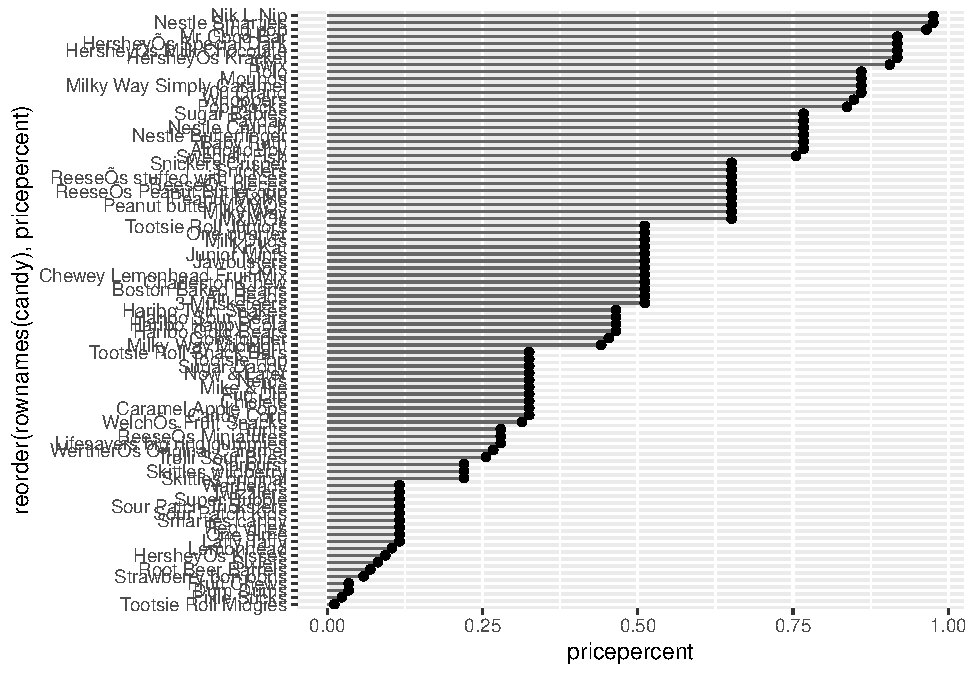
\includegraphics{Vaccination-Rates-Mini-Project_files/figure-latex/unnamed-chunk-21-1.pdf}

\hypertarget{focus-on-ucsdla-jolla}{%
\section{Focus on UCSD/La Jolla}\label{focus-on-ucsdla-jolla}}

UC San Diego resides in the 92037 ZIP code area and is listed with an
age 5+ population size of 36,144.

\begin{Shaded}
\begin{Highlighting}[]
\NormalTok{ucsd }\OtherTok{\textless{}{-}} \FunctionTok{filter}\NormalTok{(sd, zip\_code\_tabulation\_area}\SpecialCharTok{==}\StringTok{"92037"}\NormalTok{)}
\NormalTok{ucsd[}\DecValTok{1}\NormalTok{,]}\SpecialCharTok{$}\NormalTok{age5\_plus\_population}
\end{Highlighting}
\end{Shaded}

\begin{verbatim}
## [1] 36144
\end{verbatim}

\textbf{Q15}. Using ggplot make a graph of the vaccination rate time
course for the 92037 ZIP code area:

\begin{Shaded}
\begin{Highlighting}[]
\FunctionTok{library}\NormalTok{(ggplot2)}
\FunctionTok{ggplot}\NormalTok{(ucsd) }\SpecialCharTok{+}
  \FunctionTok{aes}\NormalTok{(as\_of\_date,}
\NormalTok{      percent\_of\_population\_fully\_vaccinated) }\SpecialCharTok{+}
  \FunctionTok{geom\_point}\NormalTok{() }\SpecialCharTok{+}
  \FunctionTok{geom\_line}\NormalTok{(}\AttributeTok{group=}\DecValTok{1}\NormalTok{) }\SpecialCharTok{+}
  \FunctionTok{ylim}\NormalTok{(}\FunctionTok{c}\NormalTok{(}\DecValTok{0}\NormalTok{,}\DecValTok{1}\NormalTok{)) }\SpecialCharTok{+}
  \FunctionTok{labs}\NormalTok{(}\AttributeTok{x=}\StringTok{"Date"}\NormalTok{, }\AttributeTok{y=}\StringTok{"Percent Vaccinated"}\NormalTok{)}
\end{Highlighting}
\end{Shaded}

\includegraphics{Vaccination-Rates-Mini-Project_files/figure-latex/unnamed-chunk-23-1.pdf}
This plot shows an initial slow roll out in January into Febuary (likely
due to limited vaccine availability). This is followed with rapid ramp
up until a clear slowing trend from June time onward. Interpertation
beyond this requies context from other zip code areas to answer
questions such as: is this trend representative of other areas? Are more
people fully vaccinated in this area compared to others? Etc.

\hypertarget{comparing-to-similar-sized-areas}{%
\section{Comparing to similar sized
areas}\label{comparing-to-similar-sized-areas}}

Let's return to the full dataset and look across every zip code area
with a population at least as large as that of 92037 on as\_of\_date
``2021-11-16''.

\begin{Shaded}
\begin{Highlighting}[]
\CommentTok{\# Subset to all CA areas with a population as large as 92037}
\NormalTok{vax}\FloatTok{.36} \OtherTok{\textless{}{-}} \FunctionTok{filter}\NormalTok{(vax, age5\_plus\_population }\SpecialCharTok{\textgreater{}} \DecValTok{36144} \SpecialCharTok{\&}
\NormalTok{                as\_of\_date }\SpecialCharTok{==} \StringTok{"2021{-}11{-}16"}\NormalTok{)}
\FunctionTok{head}\NormalTok{(vax}\FloatTok{.36}\NormalTok{)}
\end{Highlighting}
\end{Shaded}

\begin{verbatim}
##   as_of_date zip_code_tabulation_area local_health_jurisdiction         county
## 1 2021-11-16                    92020                 San Diego      San Diego
## 2 2021-11-16                    92563                 Riverside      Riverside
## 3 2021-11-16                    92806                    Orange         Orange
## 4 2021-11-16                    93291                    Tulare         Tulare
## 5 2021-11-16                    92335            San Bernardino San Bernardino
## 6 2021-11-16                    92618                    Orange         Orange
##   vaccine_equity_metric_quartile                 vem_source
## 1                              2 Healthy Places Index Score
## 2                              3 Healthy Places Index Score
## 3                              2 Healthy Places Index Score
## 4                              1 Healthy Places Index Score
## 5                              1 Healthy Places Index Score
## 6                              4 Healthy Places Index Score
##   age12_plus_population age5_plus_population persons_fully_vaccinated
## 1               49284.5                54991                    35128
## 2               55897.8                63794                    36051
## 3               33050.9                36739                    24810
## 4               46879.7                54254                    27936
## 5               79670.3                91867                    49820
## 6               40348.0                44304                    39695
##   persons_partially_vaccinated percent_of_population_fully_vaccinated
## 1                         5161                               0.638795
## 2                         4224                               0.565116
## 3                         2355                               0.675304
## 4                         4012                               0.514911
## 5                         5970                               0.542306
## 6                         3936                               0.895969
##   percent_of_population_partially_vaccinated
## 1                                   0.093852
## 2                                   0.066213
## 3                                   0.064101
## 4                                   0.073948
## 5                                   0.064985
## 6                                   0.088841
##   percent_of_population_with_1_plus_dose redacted
## 1                               0.732647       No
## 2                               0.631329       No
## 3                               0.739405       No
## 4                               0.588859       No
## 5                               0.607291       No
## 6                               0.984810       No
\end{verbatim}

\textbf{Q16}. Calculate the mean ``Percent of Population Fully
Vaccinated'' for ZIP code areas with a population as large as 92037 (La
Jolla) as\_of\_date ``2021-11-16''. Add this as a straight horizontal
line to your plot from above with the geom\_hline() function?

\begin{Shaded}
\begin{Highlighting}[]
\FunctionTok{mean}\NormalTok{(vax}\FloatTok{.36}\SpecialCharTok{$}\NormalTok{percent\_of\_population\_fully\_vaccinated)}
\end{Highlighting}
\end{Shaded}

\begin{verbatim}
## [1] 0.6640413
\end{verbatim}

Let's make a new plot:

\begin{Shaded}
\begin{Highlighting}[]
\NormalTok{ucsd}\SpecialCharTok{$}\NormalTok{as\_of\_date}
\end{Highlighting}
\end{Shaded}

\begin{verbatim}
##  [1] "2021-01-05" "2021-01-12" "2021-01-19" "2021-01-26" "2021-02-02"
##  [6] "2021-02-09" "2021-02-16" "2021-02-23" "2021-03-02" "2021-03-09"
## [11] "2021-03-16" "2021-03-23" "2021-03-30" "2021-04-06" "2021-04-13"
## [16] "2021-04-20" "2021-04-27" "2021-05-04" "2021-05-11" "2021-05-18"
## [21] "2021-05-25" "2021-06-01" "2021-06-08" "2021-06-15" "2021-06-22"
## [26] "2021-06-29" "2021-07-06" "2021-07-13" "2021-07-20" "2021-07-27"
## [31] "2021-08-03" "2021-08-10" "2021-08-17" "2021-08-24" "2021-08-31"
## [36] "2021-09-07" "2021-09-14" "2021-09-21" "2021-09-28" "2021-10-05"
## [41] "2021-10-12" "2021-10-19" "2021-10-26" "2021-11-02" "2021-11-09"
## [46] "2021-11-16" "2021-11-23"
\end{verbatim}

\begin{Shaded}
\begin{Highlighting}[]
\FunctionTok{ggplot}\NormalTok{(ucsd) }\SpecialCharTok{+}
  \FunctionTok{aes}\NormalTok{(as\_of\_date, }
\NormalTok{  percent\_of\_population\_fully\_vaccinated) }\SpecialCharTok{+}
  \FunctionTok{geom\_point}\NormalTok{() }\SpecialCharTok{+}
  \FunctionTok{geom\_line}\NormalTok{(}\AttributeTok{group=}\DecValTok{1}\NormalTok{) }\SpecialCharTok{+}
  \FunctionTok{ylim}\NormalTok{(}\FunctionTok{c}\NormalTok{(}\DecValTok{0}\NormalTok{,}\DecValTok{1}\NormalTok{)) }\SpecialCharTok{+}
  \FunctionTok{labs}\NormalTok{(}\AttributeTok{x=}\StringTok{"Date"}\NormalTok{, }\AttributeTok{y=}\StringTok{"Percent Vaccinated"}\NormalTok{) }\SpecialCharTok{+}
  \FunctionTok{geom\_hline}\NormalTok{(}\AttributeTok{yintercept =} \FloatTok{0.6640413}\NormalTok{)}
\end{Highlighting}
\end{Shaded}

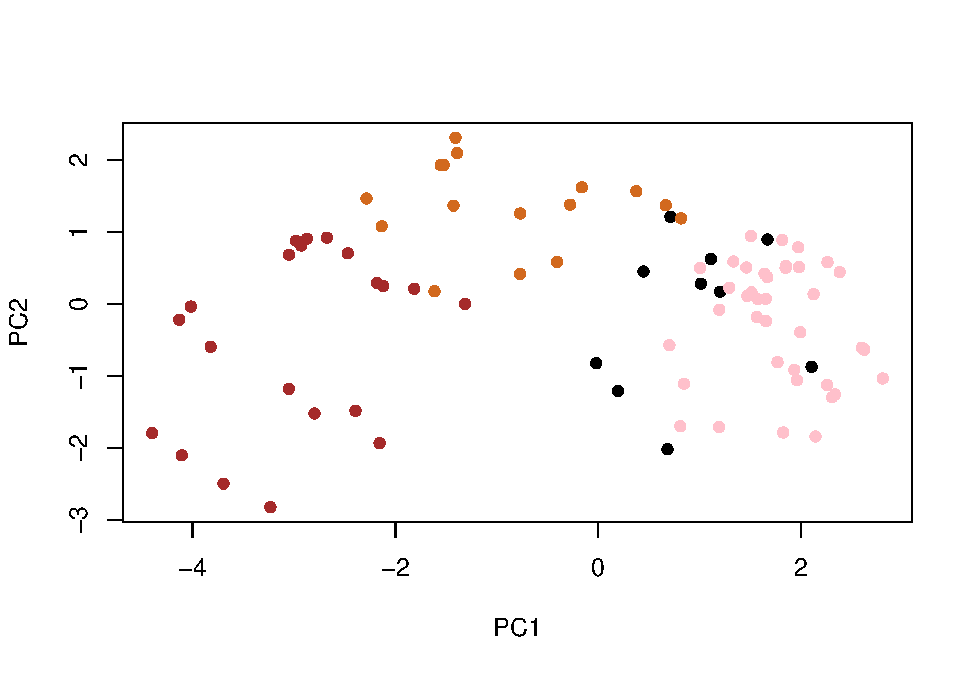
\includegraphics{Vaccination-Rates-Mini-Project_files/figure-latex/unnamed-chunk-26-1.pdf}

\textbf{Q17}. What is the 6 number summary (Min, 1st Qu., Median, Mean,
3rd Qu., and Max) of the ``Percent of Population Fully Vaccinated''
values for ZIP code areas with a population as large as 92037 (La Jolla)
as\_of\_date ``2021-11-16''?

\begin{Shaded}
\begin{Highlighting}[]
\NormalTok{dat }\OtherTok{\textless{}{-}} \FunctionTok{summary}\NormalTok{(vax}\FloatTok{.36}\SpecialCharTok{$}\NormalTok{percent\_of\_population\_fully\_vaccinated)}
\FunctionTok{head}\NormalTok{(dat)}
\end{Highlighting}
\end{Shaded}

\begin{verbatim}
##      Min.   1st Qu.    Median      Mean   3rd Qu.      Max. 
## 0.3528910 0.5905170 0.6661630 0.6640413 0.7297545 1.0000000
\end{verbatim}

\textbf{Q18}. Using \texttt{ggplot}, generate a histogram of this data.

\begin{Shaded}
\begin{Highlighting}[]
\NormalTok{vax}\FloatTok{.36}\SpecialCharTok{$}\NormalTok{percent\_of\_population\_fully\_vaccinated}
\end{Highlighting}
\end{Shaded}

\begin{verbatim}
##   [1] 0.638795 0.565116 0.675304 0.514911 0.542306 0.895969 0.610183 0.754831
##   [9] 0.671440 0.685062 0.571825 0.685009 0.789706 0.758088 0.758018 0.668217
##  [17] 0.533796 0.651510 0.687135 0.672017 0.705095 0.765967 0.544121 0.829537
##  [25] 0.637903 0.700493 0.613925 0.628329 0.642227 0.654824 0.631281 0.682419
##  [33] 0.819272 0.730465 0.573062 0.875929 0.659628 0.511820 0.706522 0.671575
##  [41] 0.709131 0.526173 0.721366 0.821927 0.556778 0.536308 0.512772 0.674613
##  [49] 0.690915 0.589145 0.661266 0.818517 0.703561 0.556520 0.756571 0.867086
##  [57] 0.556596 0.698836 0.636051 0.777597 0.625551 0.631382 0.716066 0.588702
##  [65] 0.539396 0.707375 0.718392 0.472181 0.528009 0.796706 0.644050 0.783687
##  [73] 0.631097 0.956078 0.753598 0.547531 0.597529 0.480697 0.618461 0.688234
##  [81] 0.610172 0.881642 0.836037 0.649573 0.565566 0.532163 0.795321 0.687544
##  [89] 0.671494 0.542527 0.548829 0.573898 0.687350 0.878852 0.666937 0.841436
##  [97] 0.637505 0.562748 0.677776 0.700007 0.572831 0.606870 0.553326 0.714489
## [105] 0.537228 0.750175 0.563423 0.745997 0.643037 0.749612 0.623749 0.680768
## [113] 0.767511 0.521701 0.522434 0.682254 0.523732 0.583474 0.653602 0.741917
## [121] 0.764800 0.855271 0.721193 0.701577 0.500653 0.433647 0.688582 0.631672
## [129] 0.662798 0.576452 0.601809 0.542173 0.619857 0.685675 0.716349 0.637176
## [137] 0.667082 0.780244 0.541241 0.741907 0.517657 0.685097 0.670161 0.707103
## [145] 0.767342 0.733755 0.638490 0.716598 0.759017 0.601673 0.702513 0.655895
## [153] 0.640323 0.768993 0.839498 0.684763 0.652456 0.517969 0.654527 0.654024
## [161] 0.530940 0.764964 0.742775 0.805337 0.651185 0.721270 0.614656 0.695125
## [169] 0.859553 0.728817 0.628313 0.670734 0.656297 0.764209 0.756293 0.948087
## [177] 0.690923 0.485393 0.574872 0.510786 0.610938 0.577006 0.549621 0.651296
## [185] 0.569071 0.788966 0.463319 0.623384 0.717695 0.784795 1.000000 0.658827
## [193] 0.574434 0.530863 0.654740 0.755299 0.586125 0.645119 0.436113 0.715121
## [201] 0.524522 0.657273 0.605903 0.665958 0.493331 0.771810 0.656647 0.526546
## [209] 0.603002 0.686999 0.476319 0.556440 0.668021 0.763976 0.632720 0.541915
## [217] 0.666057 0.714168 0.556318 0.743329 0.755339 0.811226 0.616480 0.813719
## [225] 0.595697 0.602320 0.653758 0.573314 0.758939 0.795904 0.620828 0.672871
## [233] 0.851894 0.584296 0.633778 0.521047 0.611774 0.784453 0.818396 0.557832
## [241] 0.549247 0.655007 0.776212 0.908691 0.842151 0.706651 0.522779 0.671247
## [249] 0.849087 0.661316 0.568585 0.552498 0.429913 0.741157 0.683580 0.518647
## [257] 0.778177 0.703912 0.530206 0.772152 0.584391 0.665908 0.820835 0.712352
## [265] 0.786689 0.704918 0.525192 0.591063 0.691787 0.775898 0.815766 0.634499
## [273] 0.686369 0.641569 0.620949 0.628331 0.749648 0.782176 0.674917 0.613536
## [281] 0.733390 0.662913 0.717260 0.708893 0.596023 0.703498 0.625933 0.750124
## [289] 0.634371 0.680762 0.669844 0.666881 0.702129 0.647831 0.844584 0.703221
## [297] 0.644819 0.602026 0.671617 0.778482 0.450352 0.696519 0.670376 0.566692
## [305] 0.666163 0.747186 0.504311 0.726094 0.798128 0.529317 0.742954 0.729044
## [313] 0.978329 0.695313 0.663354 0.603575 0.620572 0.632964 0.718851 0.611506
## [321] 0.564079 0.839156 0.821020 0.784338 0.789746 0.764371 0.546735 0.521949
## [329] 0.616061 0.667899 0.508542 0.781801 0.546277 0.628636 0.518007 0.786246
## [337] 0.676550 0.590092 0.707749 0.680295 0.590942 0.532132 0.747721 0.599918
## [345] 0.690365 0.352891 0.562106 0.468672 0.616078 0.541572 0.723034 0.591270
## [353] 0.727442 0.680905 0.653183 0.819011 0.692538 0.788603 0.454901 0.713177
## [361] 0.708313 0.489985 0.732898 0.640603 0.594066 0.619922 0.651024 0.860438
## [369] 0.671776 0.718488 0.496700 0.754363 0.589222 0.746015 0.668050 0.701483
## [377] 0.615606 0.609210 0.809691 0.544870 0.625113 0.610835 0.576914 0.694395
## [385] 0.763135 0.619944 0.649547 0.651101 0.613572 0.694361 0.839469 0.760372
## [393] 0.744376 0.680805 0.688630 0.604627 0.715254 0.524380 0.576548 0.668389
## [401] 0.818129 0.498205 0.544950 0.790066 0.524256 0.703243 0.708919 0.561631
## [409] 0.572598 0.692633 0.799640
\end{verbatim}

\begin{Shaded}
\begin{Highlighting}[]
\FunctionTok{ggplot}\NormalTok{(vax}\FloatTok{.36}\NormalTok{) }\SpecialCharTok{+}
  \FunctionTok{aes}\NormalTok{(vax}\FloatTok{.36}\SpecialCharTok{$}\NormalTok{percent\_of\_population\_fully\_vaccinated) }\SpecialCharTok{+}
  \FunctionTok{geom\_histogram}\NormalTok{()}
\end{Highlighting}
\end{Shaded}

\begin{verbatim}
## Warning: Use of `vax.36$percent_of_population_fully_vaccinated` is discouraged.
## Use `percent_of_population_fully_vaccinated` instead.
\end{verbatim}

\begin{verbatim}
## `stat_bin()` using `bins = 30`. Pick better value with `binwidth`.
\end{verbatim}

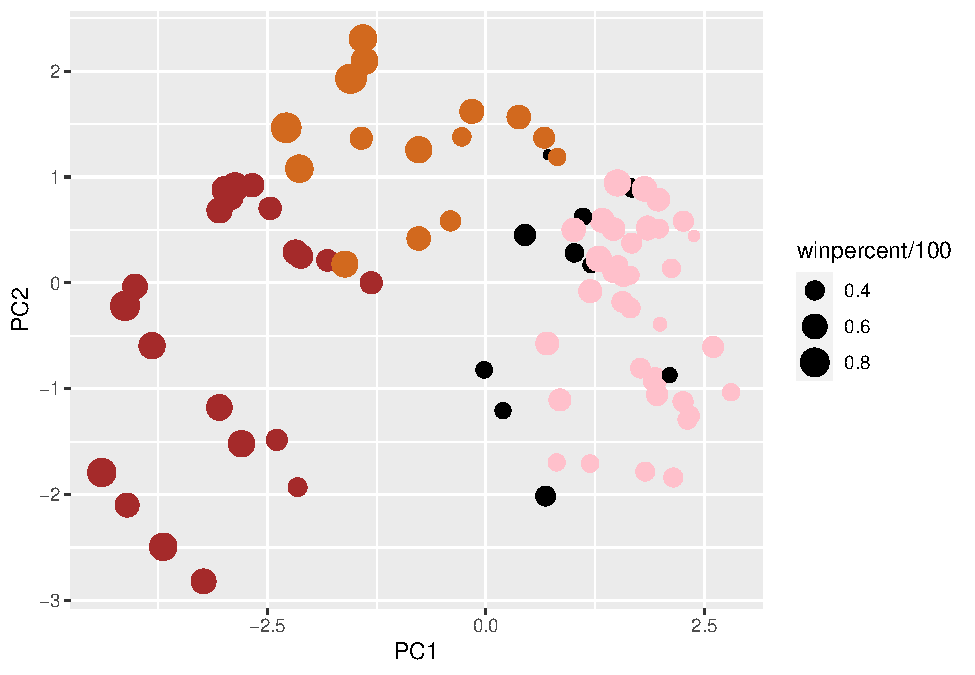
\includegraphics{Vaccination-Rates-Mini-Project_files/figure-latex/unnamed-chunk-28-1.pdf}

\textbf{Q19}. Is the 92109 and 92040 ZIP code areas above or below the
average value you calculated for all these above?

\begin{Shaded}
\begin{Highlighting}[]
\NormalTok{vax }\SpecialCharTok{\%\textgreater{}\%} \FunctionTok{filter}\NormalTok{(as\_of\_date }\SpecialCharTok{==} \StringTok{"2021{-}11{-}16"}\NormalTok{) }\SpecialCharTok{\%\textgreater{}\%}  
  \FunctionTok{filter}\NormalTok{(zip\_code\_tabulation\_area}\SpecialCharTok{==}\StringTok{"92040"}\NormalTok{) }\SpecialCharTok{\%\textgreater{}\%}
  \FunctionTok{select}\NormalTok{(percent\_of\_population\_fully\_vaccinated)}
\end{Highlighting}
\end{Shaded}

\begin{verbatim}
##   percent_of_population_fully_vaccinated
## 1                               0.521047
\end{verbatim}

\begin{Shaded}
\begin{Highlighting}[]
\NormalTok{vax }\SpecialCharTok{\%\textgreater{}\%} \FunctionTok{filter}\NormalTok{(as\_of\_date }\SpecialCharTok{==} \StringTok{"2021{-}11{-}16"}\NormalTok{) }\SpecialCharTok{\%\textgreater{}\%}  
  \FunctionTok{filter}\NormalTok{(zip\_code\_tabulation\_area}\SpecialCharTok{==}\StringTok{"92109"}\NormalTok{) }\SpecialCharTok{\%\textgreater{}\%}
  \FunctionTok{select}\NormalTok{(percent\_of\_population\_fully\_vaccinated)}
\end{Highlighting}
\end{Shaded}

\begin{verbatim}
##   percent_of_population_fully_vaccinated
## 1                                0.68863
\end{verbatim}

--\textgreater{} 92109 ZIP code = above, 92040 ZIP code = below

\textbf{Q20}. Finally, make a time course plot of vaccination progress
for all areas in the full dataset with a age5\_plus\_population
\textgreater{} 36144.

\begin{Shaded}
\begin{Highlighting}[]
\NormalTok{vax.}\FloatTok{36.}\NormalTok{all }\OtherTok{\textless{}{-}} \FunctionTok{filter}\NormalTok{(vax, age5\_plus\_population }\SpecialCharTok{\textgreater{}} \DecValTok{36144}\NormalTok{)}
\FunctionTok{ggplot}\NormalTok{(vax.}\FloatTok{36.}\NormalTok{all) }\SpecialCharTok{+}
  \FunctionTok{aes}\NormalTok{(as\_of\_date,}
\NormalTok{      percent\_of\_population\_fully\_vaccinated, }
      \AttributeTok{group=}\NormalTok{zip\_code\_tabulation\_area) }\SpecialCharTok{+}
  \FunctionTok{geom\_line}\NormalTok{(}\AttributeTok{alpha=}\FloatTok{0.2}\NormalTok{, }\AttributeTok{color=}\StringTok{"purple"}\NormalTok{) }\SpecialCharTok{+}
  \FunctionTok{ylim}\NormalTok{(}\FunctionTok{c}\NormalTok{(}\DecValTok{0}\NormalTok{,}\DecValTok{1}\NormalTok{)) }\SpecialCharTok{+}
  \FunctionTok{labs}\NormalTok{(}\AttributeTok{x=}\StringTok{"Date"}\NormalTok{, }\AttributeTok{y=}\StringTok{"Percent Vaccinated"}\NormalTok{,}
       \AttributeTok{title=}\StringTok{"Vaccination Rate Across California"}\NormalTok{,}
       \AttributeTok{subtitle=}\StringTok{"Only areas with a population about 36K are shown"}\NormalTok{) }\SpecialCharTok{+}
  \FunctionTok{geom\_hline}\NormalTok{(}\AttributeTok{yintercept =} \FloatTok{0.6629812}\NormalTok{, }\AttributeTok{linetype =} \StringTok{"dashed"}\NormalTok{)}
\end{Highlighting}
\end{Shaded}

\begin{verbatim}
## Warning: Removed 176 row(s) containing missing values (geom_path).
\end{verbatim}

\includegraphics{Vaccination-Rates-Mini-Project_files/figure-latex/unnamed-chunk-30-1.pdf}

\textbf{Q21}. How do you feel about traveling for Thanksgiving and
meeting for in-person class next week?

--\textgreater{} I missed our in-person class this week due to travel
plans, but was able to work through the mini-project :)

\end{document}
